\section{Describing the YoungDrive Coaches and the Research Context}

The biggest challenge with regards to time constraints and cultural differences is that it is difficult to understand the target group of the app. Therefore, the whole design and development process will take place in Uganda, with several interactions with the intended users. The work was carried out from Hive Colab, a co-working space and an innovation hub. The work is done mainly from Kampala, because that is where YoungDrive is situated, meaning that there is still a long distance to the coaches and youth in Tororo, which is located near the Kenyan border. Another challenge with being in Uganda compared to Sweden is that internet speed and access is worse, especially outside Kampala.

 The interactions took place in either Uganda or Zambia, in the locations where training of the coaches and youth takes place.  There were a number of resources made available to support the work, for example the YoungDrive manuals. Each youth is given a \textit{Participant manual}, describing each week of the 10-week YoungDrive program. Coaches are also given a \textit{Coach guide}, which describes how to carry out and teach each week's topic during the youth training. As most of the coaches did not have smartphones or tablets, four smartphones (3 Android, 1 iOS) and ten tablets (3 Android, 7 iOS) were brought from Sweden. All of these devices had a web browser and access to an app store. These were either donated, borrowed or bought devices. During the user tests, also using a laptop would be tested. The following section describes the Ugandian and Zambian coaches and their businesses.

\subsection{Social Characteristics and Businesses in Uganda}

According to statistics gathered by YoungDrive during 2015 evaluations \citep{youngdrive-statistics}, there are a number of considerations to make regarding the coaches in Uganda. This regards entrepreneurship experience, technical access, and language, see a summary in figure \ref{fig:ydStatistics}. Taken together the coaches' and project leaders' technical skills are currently low, and this needs to be in consideration when designing the app. Regarding language, English can be used in the coach app.

\begin{figure}[h]
    \centering
    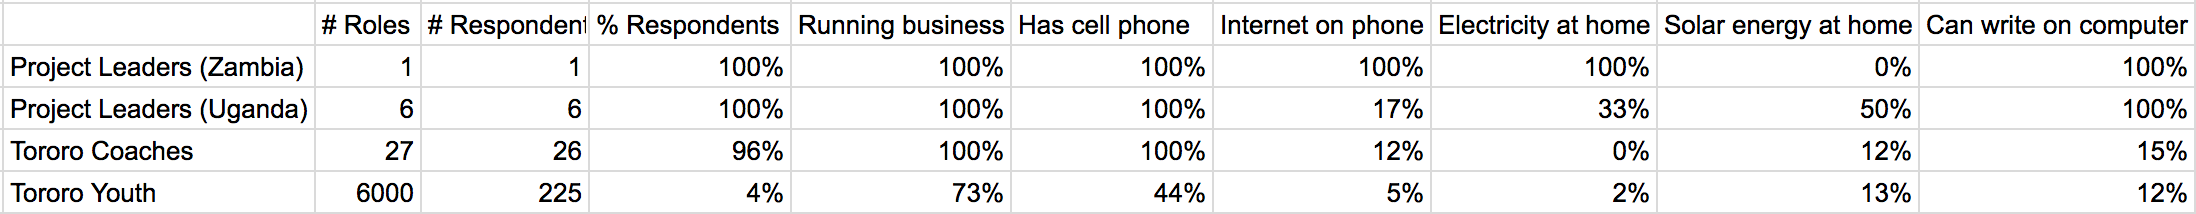
\includegraphics[width=1.0\textwidth]{ydStatistics.png}
    \caption{Table showing entrepreneurship experience, technical access, and language between Tororo coaches and the project leaders in Uganda and Zambia. All of the Tororo coaches run a business (with a majority running more than one). This means they do have practical experience of running a business outside of the YoungDrive coach training. While all have a cell phone, smartphones are very uncommon - only 3 uses Internet on the phone, every day or weekly (mostly for Facebook or email). Regarding power, none has power at home, 3/26 has solar, and only 4/26 can write on a computer. While about half of the asked Uganda youth can not understand (129/225), read (133/225) or write (132/225) English, most of the coaches in Uganda are proficient. These characteristics are similar for youth and project leaders as well.}.
    \label{fig:ydStatistics}
\end{figure}

The coaches in Tororo are divided into three different regions. Based on region, income and experience, they run different kinds of businesses. \footnote{In Uganda and Zambia, a small-scale business is typically not registered. Thus, the coaches' definition of a business can be more generous.} In Tororo, the coaches' businesses range from: pineapple, water melon, onion, chili, bakery, catering, corn, beans, fabric, plastic products, bird farm, milk, fish, ground nuts, cabbage, tomato, hairdresser, sewer, shop and rice. For photograph of the environment, see figure \ref{fig:tororo}.

\begin{figure}[h]
    \centering
    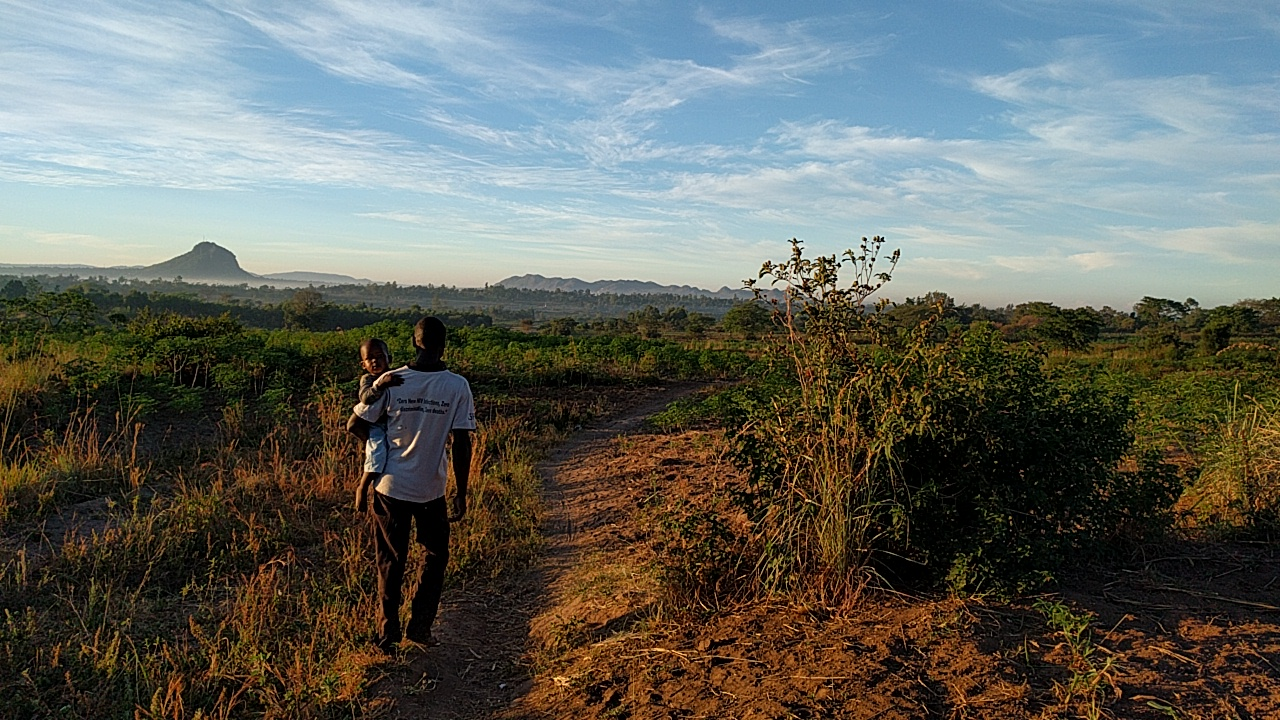
\includegraphics[width=0.7\textwidth]{stayover.jpg}
    \caption{One of the co-project leaders showing the rural part of Tororo, where crops are growing close to where he lives.}.
    \label{fig:tororo}
\end{figure}

In Tororo, there are 2 Project Leaders. one project leader's business range from: bakery, corn, pig farm and plastic products. The other person's business range from: silver fish, beans, corn, and bird farm. In comparison, in Kamuli, there are 4 Project Leaders. Their businesses range from: selling office supply, motorcycle taxi, bird farm, pig farm, green pepper, corn, cabbage, tomato, aubergine, chipati ("bread"), chilli, and charging of cellphones.

Among the youth, the top 8 most popular businesses in Tororo, with 134 respondents, are corn, cassava ("potato"), saloon, fish, making of bricks, beans, brooms and rope. These range from 9 for corn (6.7\%) to 5 for rope (3.7\%).

\subsection{Social Characteristics and Businesses in Zambia}
During the visit in Zambia, the coaches had not yet formed their youth groups, and started their own teaching. Regarding characteristics, ages ranged from 21-39 years old (26.8 average). Other data available about the coaches were notes of the Zambian coach job interviews, which could be compared with during quiz analysis \citep{yd-zambia-interviews}. Compared with Uganda, 9 out of 10 had business experience.

%3 were mentioned as being shy during the interviews. They lived from 10-90 minutes outside of town (33 minutes average).

%Regarding motivations for being a coach, 50\% had an emphasis on benefiting the community, and 90\% had personal reasons.



%Care for oneself:
%\begin{itemize}
%\item Learn business %(7)
%\item More skills %(2)
%\item Get idea
%\item Expand business
%\item Benefit CV
%\end{itemize}
%
%Care for community:
%\begin{itemize}
%\item Empower %(2)
%\item Teach business
%\item Leadership
%\item Share
%\item Stop bad behaviours of youth
%\end{itemize}

%regarding experience, 8 had trained youth before, 8 had been a leader before, 9 had business experience. Regarding YoungDrive, they said they could handle training between 8-30 youth (19.8 on average) per group. They could have 1-5 groups per coach (average 3.0), totalling a range between 8-101.5 youth (average 59.8).
